\chapter{Result Analysis}

\section{Performance Evaluation}\label{sec:evaluation}

\subsection{Testing Method}\label{sec:testing}

The framework and the retraining strategies are tested by replaying each dataset in strict time order, as described in Section \ref{sec:overview}. A model is trained on the history, deployed at the start of the stream and scores each following week before the labels of that week are known; the labels become usable only after the label delay of 0, 15, 30 or 60 days. Every strategy starts from the same initial model and sees exactly the same data, so differences between strategies come only from their retraining decisions. The framework itself is tested by a full replay with its registry, monitor and promotion gate (Section \ref{sec:replay5}) and by injecting faults into its retraining jobs (Section \ref{sec:faults5}).

\subsection{Evaluation Metrics}\label{sec:metrics}

The main metric is the mean weekly PR-AUC (Equation \ref{eq:weekly}), computed per week so that scores of different model versions are never pooled. ROC-AUC, precision, recall and F1 at each model's validation threshold, the lowest weekly PR-AUC and the number of retrains are reported as secondary measures. Drift is measured with the PSI (Equation \ref{eq:psi}). Differences between strategies are reported with 95\% paired day-block bootstrap intervals, and a difference is called reliable when its interval excludes zero. Because the datasets differ in difficulty, a model without skill would score 0.035 on IEEE-CIS, 0.005 on Sparkov and 0.011 on BAF, so PR-AUC values are compared within a dataset only.

\subsection{Model Performance and Drift after Deployment}\label{sec:rq1}

Table \ref{tab:decay} and Figure \ref{fig:decay} show how the static model performed over the test period of each dataset, which follows the training and validation periods in time.

{\footnotesize
\begin{longtable}{>{\raggedright\arraybackslash}p{0.32\textwidth}>{\raggedright\arraybackslash}p{0.21\textwidth}>{\raggedright\arraybackslash}p{0.21\textwidth}>{\raggedright\arraybackslash}p{0.21\textwidth}}
\caption{Performance of the static model and drift of its inputs after deployment}\label{tab:decay}\\
\toprule
\textbf{} & \textbf{IEEE-CIS} & \textbf{Sparkov} & \textbf{BAF} \\
\midrule
\endfirsthead
\toprule
\textbf{} & \textbf{IEEE-CIS} & \textbf{Sparkov} & \textbf{BAF} \\
\midrule
\endhead
PR-AUC over the whole test period & 0.510 & 0.936 & 0.164 \\ \midrule
ROC-AUC over the whole test period & 0.888 & 0.997 & 0.871 \\ \midrule
PR-AUC, first time bin & 0.581 & 0.954 & 0.164 \\ \midrule
PR-AUC, lowest time bin & 0.388 (bin 6) & 0.893 (bin 10) & 0.149 (bin 6) \\ \midrule
PR-AUC, last time bin & 0.534 & 0.893 & 0.169 \\ \midrule
Largest feature PSI (feature) & 0.17 (D10) & 0.53 (card\_txns\_24h) & 4.60 (velocity\_4w) \\ \midrule
Score-PSI trigger (threshold 0.1) & never fired; maximum score PSI 0.017 & fired once (1 of 4 label delays) & never fired \\ \bottomrule
\end{longtable}
}

\begin{figure}[htbp]
  \centering
  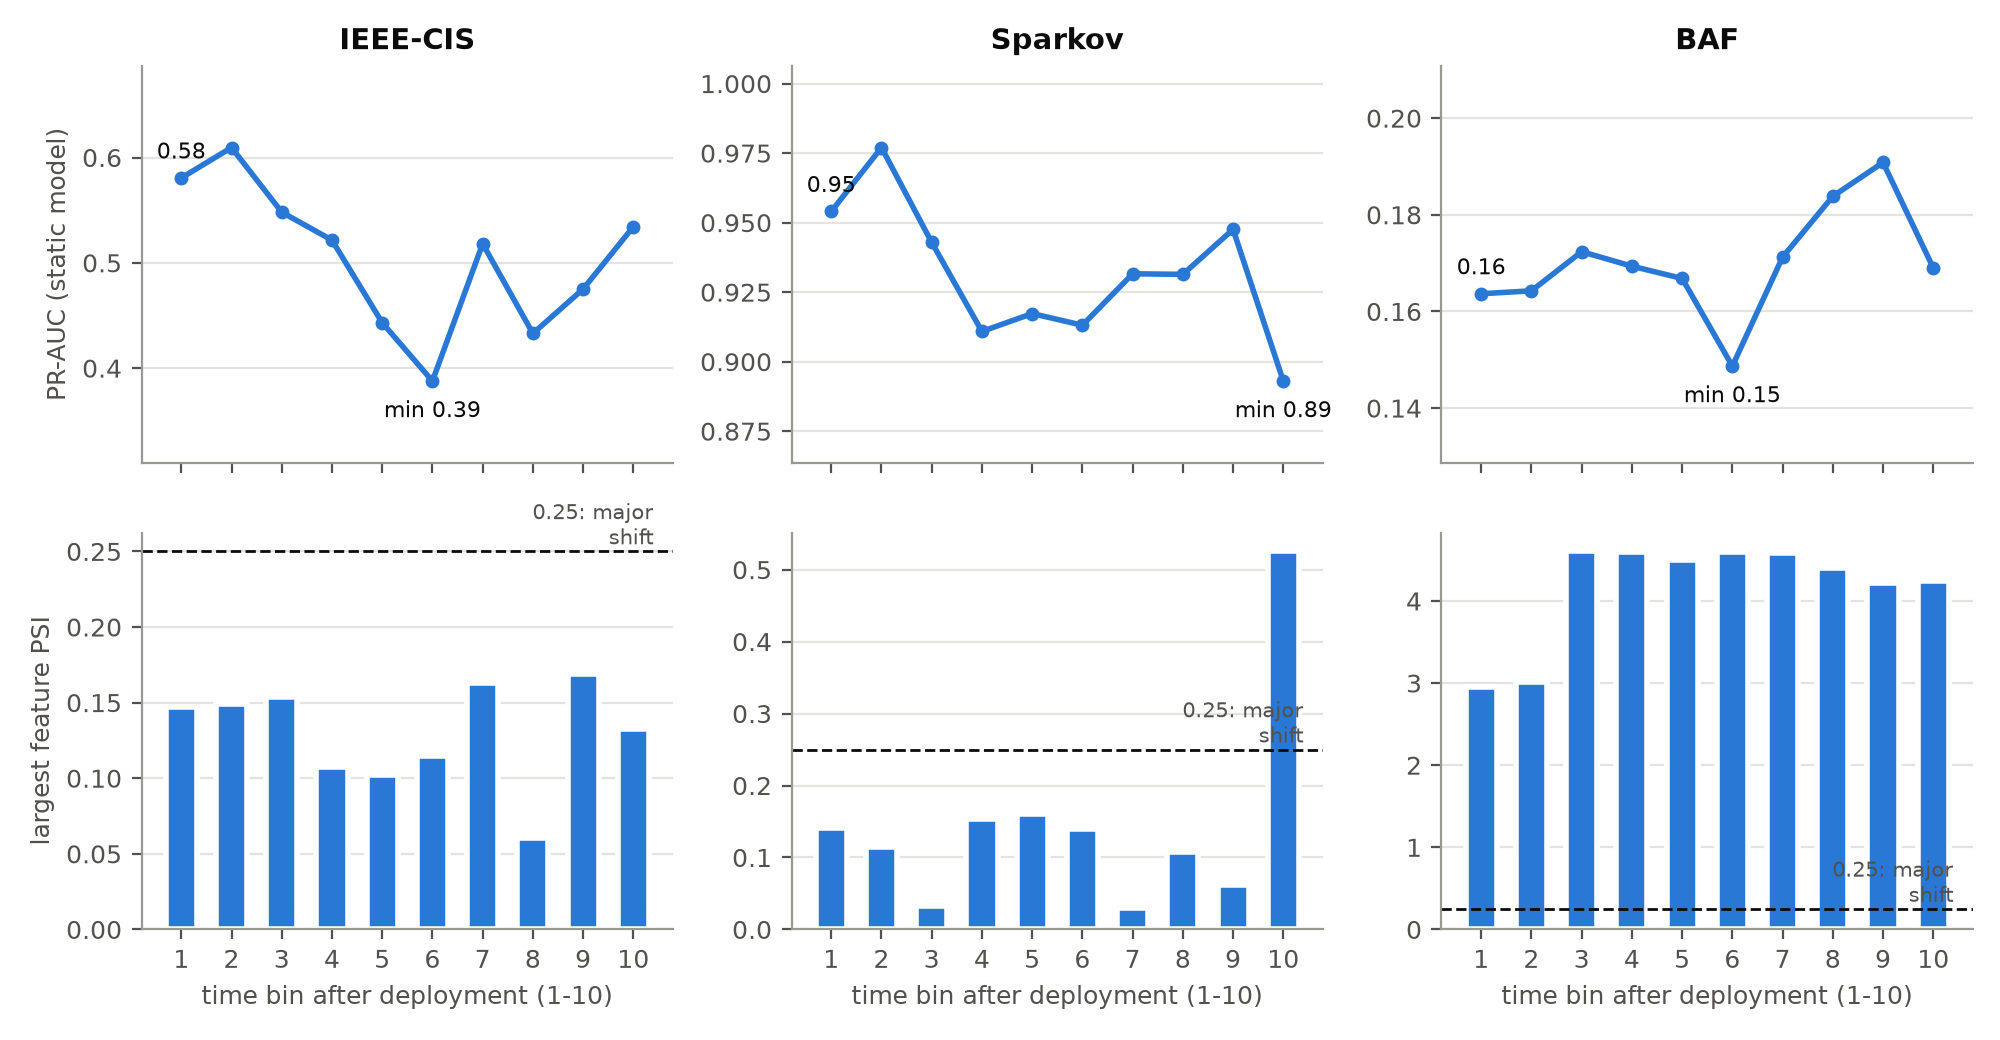
\includegraphics[width=\textwidth]{figures/results_decay.png}
  \caption{Static model after deployment, in ten consecutive time bins of the test period: PR-AUC (top) and the largest PSI among the ten most important features (bottom). Each panel has its own scale}
  \label{fig:decay}
\end{figure}

\textbf{IEEE-CIS decays, and the drift measures do not see it.} The PR-AUC of the static model fell from 0.581 in the first time bin to 0.388 in the sixth, a relative loss of a third, before partly recovering to 0.534. ROC-AUC fell from 0.920 to 0.849 over the same bins. Over the same period, none of the ten most important features reached the 0.25 level of a major shift (the largest PSI was 0.17), and the PSI of the model's scores never exceeded 0.017. A label-free monitor would therefore have reported a stable system during the largest loss of performance in the study. This agrees with the decay that Menezes and Filho observed for graph models on the same dataset \cite{menezes2025}, and shows that the decay is not visible in the input distribution.

\textbf{Sparkov and BAF drift, and the model does not decay.} On Sparkov the per-card activity features drifted strongly in the last bin (PSI 0.53), and on BAF the velocity features shifted far beyond any usual threshold in every bin (PSI up to 4.60), yet PR-AUC stayed within 0.89 to 0.98 on Sparkov and within 0.15 to 0.19 on BAF, without a downward trend. A drift monitor on these features would have raised an alarm in almost every week. The score-PSI trigger, which looks at the model's outputs rather than its inputs, fired only once on Sparkov, at one of the four label delays, and never on BAF.

\textbf{Answer to RQ1.} The performance of a deployed fraud model can decay substantially, but whether it does depends on the data, and label-free drift measures are not a reliable indicator of it in either direction: they missed real decay on IEEE-CIS and signalled drift that did not matter on Sparkov and BAF. This is the situation that Shakil et al. anticipated when they noted that statistical drift does not always mean lower performance \cite{shakil2025}, now observed on natural drift in fraud data.

\subsection{Retraining under Label Delay}\label{sec:rq2}

Table \ref{tab:sweep} and Figure \ref{fig:delaygain} compare scheduled retraining every 14 days with the static model at label delays of 0, 15, 30 and 60 days.

{\footnotesize
\begin{longtable}{>{\raggedright\arraybackslash}p{0.12\textwidth}>{\raggedright\arraybackslash}p{0.09\textwidth}>{\raggedright\arraybackslash}p{0.12\textwidth}>{\raggedright\arraybackslash}p{0.21\textwidth}>{\raggedright\arraybackslash}p{0.21\textwidth}>{\raggedright\arraybackslash}p{0.19\textwidth}}
\caption{Gain in mean weekly PR-AUC over the static model by label delay (retraining every 14 days; 95\% intervals; bold: interval excludes zero)}\label{tab:sweep}\\
\toprule
\textbf{Dataset} & \textbf{Delay} & \textbf{Static} & \textbf{All history} & \textbf{Last 60 days} & \textbf{Drift: performance} \\
\midrule
\endfirsthead
\toprule
\textbf{Dataset} & \textbf{Delay} & \textbf{Static} & \textbf{All history} & \textbf{Last 60 days} & \textbf{Drift: performance} \\
\midrule
\endhead
IEEE-CIS & 0 d & 0.507 & \textbf{+0.033} [0.027, 0.040] & \textbf{+0.078} [0.067, 0.088] & +0.030 (2 retrains) \\ \midrule
 & 15 d & 0.491 & \textbf{+0.025} [0.020, 0.029] & \textbf{+0.062} [0.052, 0.072] & +0.020 (2) \\ \midrule
 & 30 d & 0.474 & \textbf{+0.028} [0.022, 0.033] & \textbf{+0.056} [0.046, 0.064] & +0.027 (3) \\ \midrule
 & 60 d & 0.472 & \textbf{+0.008} [0.002, 0.014] & \textbf{+0.010} [0.004, 0.016] & +0.010 (4) \\ \midrule
Sparkov & 0 d & 0.931 & \textbf{+0.016} [0.013, 0.020] & \textbf{-0.258} [-0.273, -0.242] & 0.000 (0) \\ \midrule
 & 15 d & 0.928 & \textbf{+0.017} [0.013, 0.021] & \textbf{-0.214} [-0.228, -0.199] & 0.000 (0) \\ \midrule
 & 30 d & 0.924 & \textbf{+0.019} [0.016, 0.023] & \textbf{-0.173} [-0.187, -0.160] & 0.000 (0) \\ \midrule
 & 60 d & 0.923 & \textbf{+0.019} [0.015, 0.023] & \textbf{-0.198} [-0.211, -0.183] & 0.000 (0) \\ \midrule
BAF & 0 d & 0.162 & \textbf{+0.011} [0.007, 0.015] & -0.003 [-0.007, 0.002] & 0.000 (0) \\ \midrule
 & 15 d & 0.161 & \textbf{+0.008} [0.004, 0.012] & -0.005 [-0.011, 0.000] & 0.000 (0) \\ \midrule
 & 30 d & 0.161 & \textbf{+0.009} [0.004, 0.014] & \textbf{-0.007} [-0.013, -0.002] & 0.000 (0) \\ \midrule
 & 60 d & 0.155 & \textbf{+0.010} [0.006, 0.015] & +0.002 [-0.003, 0.007] & +0.001 (1) \\ \bottomrule
\end{longtable}
}

\begin{figure}[htbp]
  \centering
  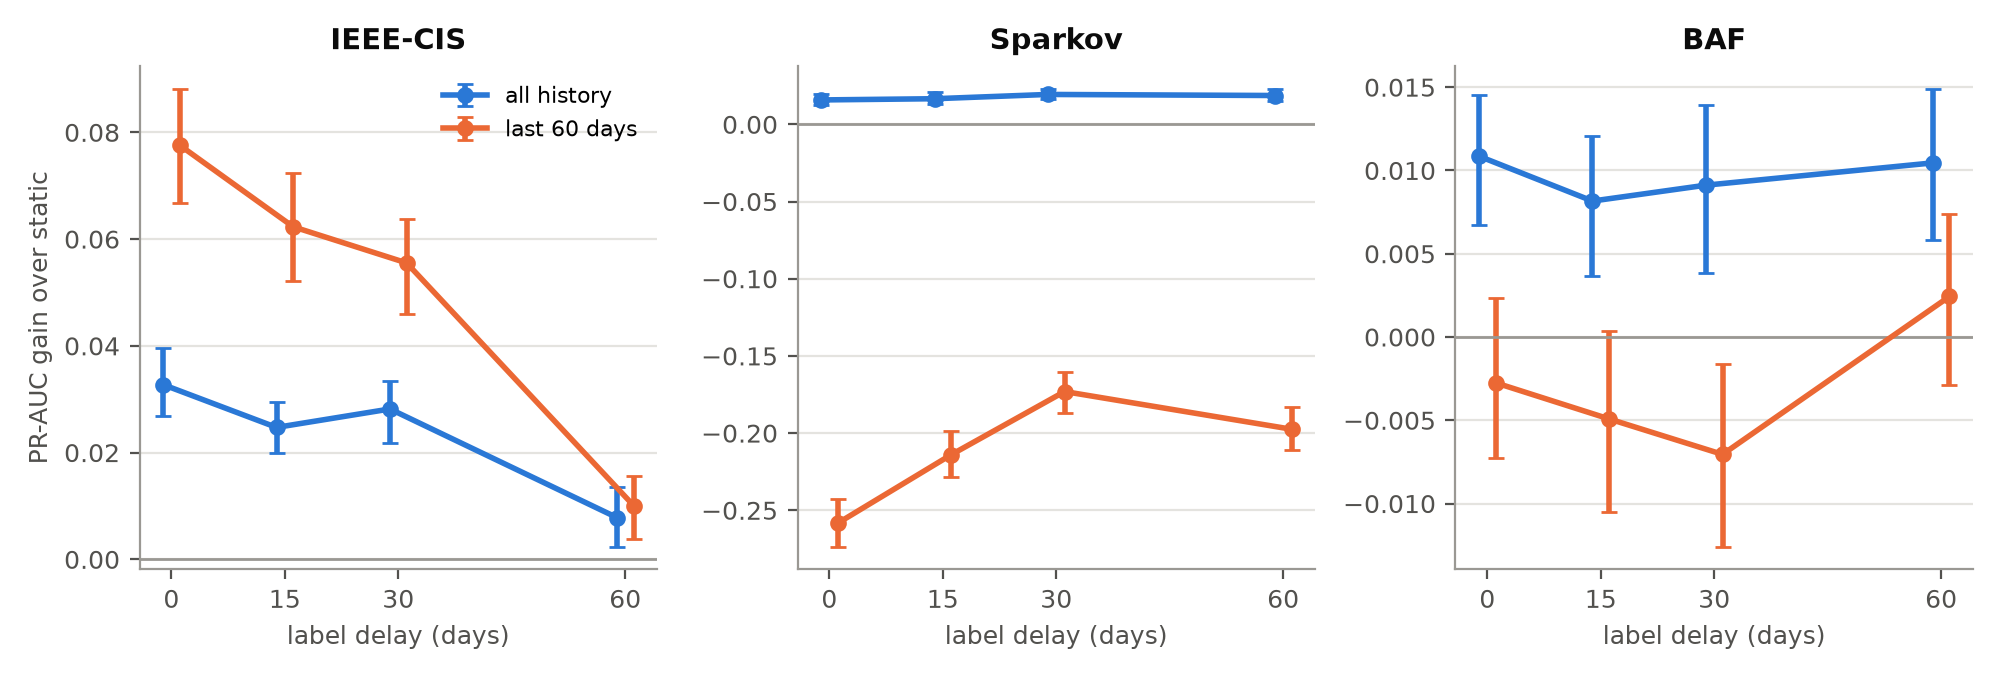
\includegraphics[width=\textwidth]{figures/results_delay.png}
  \caption{Gain in mean weekly PR-AUC over the static model for scheduled retraining every 14 days, by label delay, with 95\% paired bootstrap intervals}
  \label{fig:delaygain}
\end{figure}

\textbf{Retraining helps when its window suits the data.} On IEEE-CIS both windows improved on the static model at every delay, and the last 60 days was clearly better than all history (+0.078 against +0.033 at no delay). On Sparkov and BAF the order reversed: retraining on all history gained +0.016 to +0.019 and +0.008 to +0.011 at every delay, with every interval excluding zero, while the 60-day window was \textit{worse} than not retraining at all, dramatically so on Sparkov (-0.17 to -0.26). Sparkov has only 0.53\% fraud and a stable fraud pattern: 60 days contain too few frauds to learn it again, and the model gains nothing from forgetting older data. IEEE-CIS, in contrast, drifts, and older data teaches the model patterns that no longer hold.

\textbf{Label delay erodes the benefit.} On IEEE-CIS the gain of the 60-day window fell from +0.078 with immediate labels to +0.062 at 15 days, +0.056 at 30 days and +0.010 at 60 days, while the static model itself declined only from 0.507 to 0.472. With 60 days of delay, a retrained model learns from data that is already two months old, which on a drifting dataset is little better than the original training data. On Sparkov and BAF the gain of all-history retraining hardly changed with the delay, which is consistent with their lack of decay: when the pattern is stable, old labels are still useful.

\textbf{Untuned drift triggers rarely act.} With default settings, the performance trigger retrained two to four times on IEEE-CIS and reached between a third and half of the gain of the 60-day schedule at delays up to 30 days. On Sparkov and BAF it almost never fired, because performance never dropped by 15\%, and it behaved like the static model.

\textbf{Answer to RQ2.} Retraining improved performance on every dataset, but only with a training window that suited the data, and on the drifting dataset its benefit shrank sharply as labels arrived later; at 60 days of delay most of the benefit was gone. This confirms, on public data, the importance of verification latency stressed by Dal Pozzolo et al. \cite{dalpozzolo2018}.

\section{Analyse Design Solutions}\label{sec:analyse}

\subsection{Drift-Triggered versus Scheduled Retraining}\label{sec:rq3}

The comparison in Section \ref{sec:rq2} used default settings. Table \ref{tab:walkforward} gives the fair comparison: every family was re-tuned every four weeks with walk-forward tuning over 190 configurations, using only labels that had matured at the time.

{\footnotesize
\begin{longtable}{>{\raggedright\arraybackslash}p{0.12\textwidth}>{\raggedright\arraybackslash}p{0.08\textwidth}>{\raggedright\arraybackslash}p{0.12\textwidth}>{\raggedright\arraybackslash}p{0.16\textwidth}>{\raggedright\arraybackslash}p{0.23\textwidth}>{\raggedright\arraybackslash}p{0.22\textwidth}}
\caption{Walk-forward tuning: each family re-tuned every four weeks on matured labels only (mean weekly PR-AUC, total retrains, and differences with 95\% intervals)}\label{tab:walkforward}\\
\toprule
\textbf{Dataset} & \textbf{Delay} & \textbf{Static} & \textbf{Schedule (retrains)} & \textbf{Schedule - static} & \textbf{Drift trigger - schedule} \\
\midrule
\endfirsthead
\toprule
\textbf{Dataset} & \textbf{Delay} & \textbf{Static} & \textbf{Schedule (retrains)} & \textbf{Schedule - static} & \textbf{Drift trigger - schedule} \\
\midrule
\endhead
IEEE-CIS & 0 d & 0.470 & 0.614 (12) & \textbf{+0.144} [0.132, 0.158] & \textbf{-0.069} [-0.082, -0.060] \\ \midrule
 & 15 d & 0.468 & 0.547 (12) & \textbf{+0.079} [0.070, 0.091] & \textbf{-0.034} [-0.044, -0.027] \\ \midrule
 & 30 d & 0.458 & 0.518 (6) & \textbf{+0.059} [0.049, 0.069] & \textbf{-0.032} [-0.038, -0.025] \\ \midrule
Sparkov & 0 d & 0.916 & 0.945 (12) & \textbf{+0.029} [0.024, 0.033] & -0.001 [-0.003, 0.001] \\ \midrule
 & 15 d & 0.913 & 0.944 (12) & \textbf{+0.031} [0.026, 0.036] & \textbf{-0.007} [-0.010, -0.004] \\ \midrule
 & 30 d & 0.917 & 0.943 (12) & \textbf{+0.027} [0.023, 0.031] & \textbf{-0.007} [-0.009, -0.004] \\ \midrule
BAF & 0 d & 0.163 & 0.174 (8) & \textbf{+0.011} [0.006, 0.016] & \textbf{-0.011} [-0.016, -0.006] \\ \midrule
 & 15 d & 0.157 & 0.168 (8) & \textbf{+0.011} [0.007, 0.016] & \textbf{-0.006} [-0.011, -0.002] \\ \midrule
 & 30 d & 0.159 & 0.162 (7) & +0.003 [-0.003, 0.008] & +0.001 [-0.003, 0.006] \\ \bottomrule
\end{longtable}
}

\textbf{The tuned schedule beat or matched the tuned trigger everywhere.} On IEEE-CIS the schedule was better than the drift trigger by 0.069, 0.034 and 0.032 PR-AUC at delays of 0, 15 and 30 days, all reliable. On Sparkov the trigger came close with far fewer retrains (2 to 8 against 12): the gap was within noise with immediate labels and 0.007 at 15 and 30 days. On BAF the schedule was better at 0 and 15 days, and at 30 days neither retraining family was reliably better than the static model, because the gains on BAF are small. Of the nine comparisons, the trigger was reliably worse in seven and never reliably better.

The reason is visible in how the tuned trigger behaves under label delay. It can only react to a drop in performance after the drop has been confirmed by labels that are at least one delay old, and a drop must exceed noise in weekly PR-AUC before it is acted upon. A schedule keeps the model fresh without waiting for evidence. Where the trigger came close, as on Sparkov, it did so by retraining rarely on a stable dataset where retraining matters little.

\textbf{Answer to RQ3.} No. When both are tuned fairly and labels arrive late, drift-triggered retraining did not outperform scheduled retraining on any of the three datasets; it was worse in most comparisons and at best equal, although it retrained less often. This contradicts the results of Wong and Perumal \cite{wong2025} and Yelleti \cite{yelleti2025}, which were obtained with injected drift or immediate labels. A stronger effect than the choice of trigger was the choice of training window, which changed the result by up to 0.26 PR-AUC.

\subsection{Equal-Budget Comparison}\label{sec:budget}

Scheduled retraining retrained more often than the drift triggers in the comparisons above (for example 12 against 2 to 5 retrains in walk-forward tuning on IEEE-CIS), so part of its advantage could come simply from retraining more often. To separate the two, both families were run over many settings on IEEE-CIS and BAF, schedules every 7 days or more and 64 trigger settings, and every trigger setting was paired with the schedule that uses the same training window and the largest number of retrains that does not exceed the trigger's. The schedule therefore never has more retrains than the trigger it is compared with, which favours the trigger. Table \ref{tab:budget} summarises the pairs and Figure \ref{fig:budget} shows the best PR-AUC each family reaches within a given budget.

{\footnotesize
\begin{longtable}{>{\raggedright\arraybackslash}p{0.11\textwidth}>{\raggedright\arraybackslash}p{0.08\textwidth}>{\raggedright\arraybackslash}p{0.14\textwidth}>{\raggedright\arraybackslash}p{0.08\textwidth}>{\raggedright\arraybackslash}p{0.16\textwidth}>{\raggedright\arraybackslash}p{0.14\textwidth}>{\raggedright\arraybackslash}p{0.10\textwidth}>{\raggedright\arraybackslash}p{0.13\textwidth}}
\caption{Equal-budget comparison: each trigger setting paired with the schedule that uses the same window and no more retrains (95\% intervals; retrains: trigger / schedule)}\label{tab:budget}\\
\toprule
\textbf{Dataset} & \textbf{Delay} & \textbf{Window} & \textbf{Pairs} & \textbf{Schedule better (reliably)} & \textbf{Trigger reliably better} & \textbf{Mean diff.} & \textbf{Retrains} \\
\midrule
\endfirsthead
\toprule
\textbf{Dataset} & \textbf{Delay} & \textbf{Window} & \textbf{Pairs} & \textbf{Schedule better (reliably)} & \textbf{Trigger reliably better} & \textbf{Mean diff.} & \textbf{Retrains} \\
\midrule
\endhead
IEEE-CIS & 0 d & last 60 days & 27 & 18 (9) & 0 & +0.016 & 1.7 / 1.7 \\ \midrule
 & 30 d & last 60 days & 30 & 23 (7) & 0 & +0.011 & 2.2 / 2.2 \\ \midrule
 & 0 d & all history & 28 & 15 (14) & 0 & +0.005 & 1.7 / 1.6 \\ \midrule
 & 30 d & all history & 30 & 12 (0) & 0 & 0.000 & 2.3 / 2.2 \\ \midrule
BAF & 0 d & last 60 days & 9 & 9 (2) & 0 & +0.003 & 2.2 / 2.2 \\ \midrule
 & 30 d & last 60 days & 0 & - & - & - & trigger never fired \\ \midrule
 & 0 d & all history & 10 & 2 (1) & 3 & -0.002 & 1.9 / 1.9 \\ \midrule
 & 30 d & all history & 2 & 2 (1) & 0 & +0.004 & 2.5 / 2.5 \\ \bottomrule
\end{longtable}
}

\begin{figure}[htbp]
  \centering
  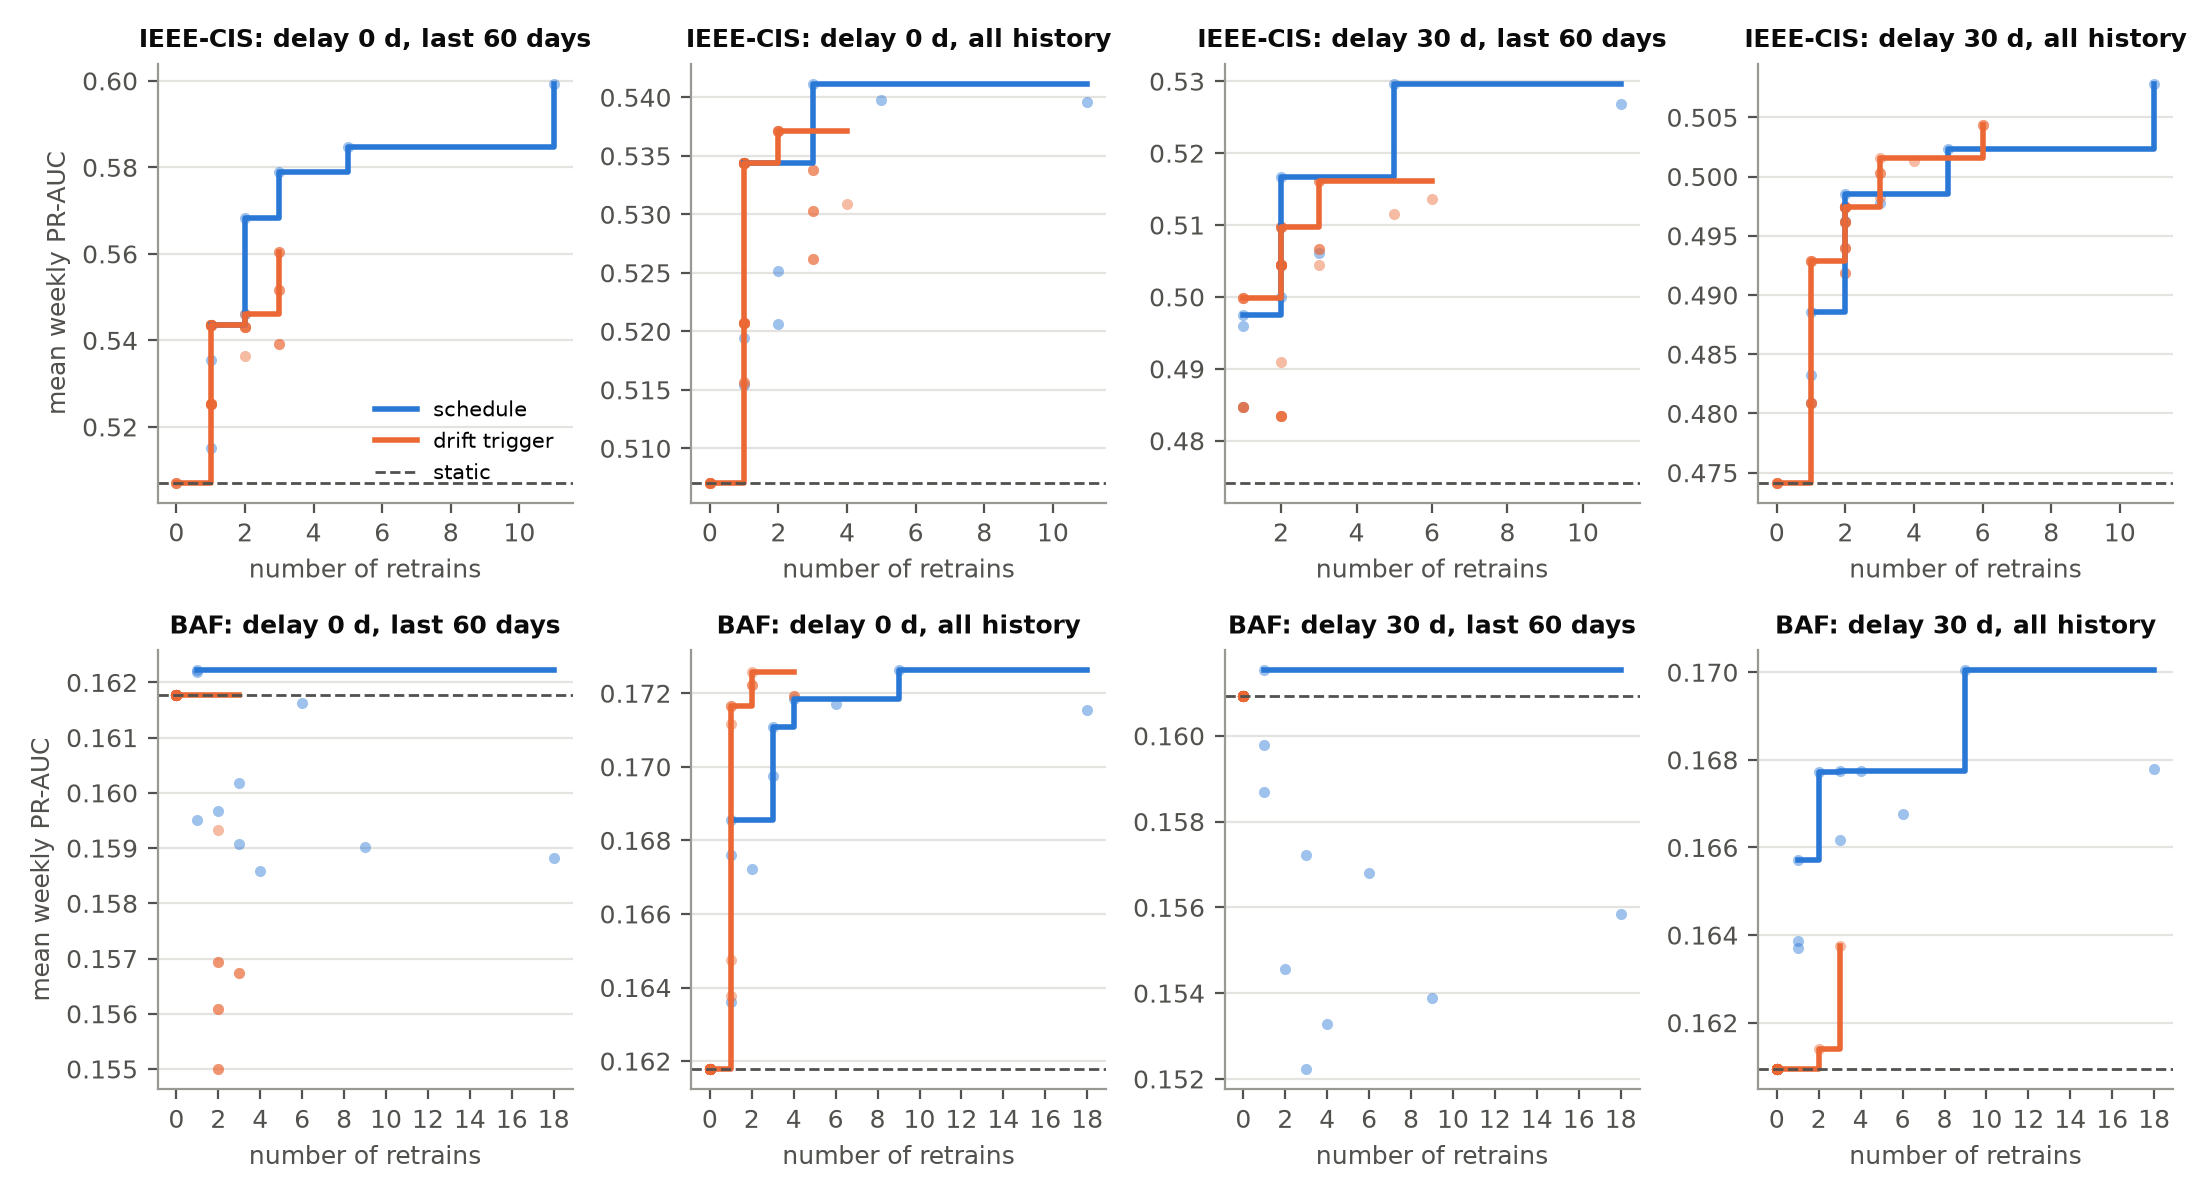
\includegraphics[width=\textwidth]{figures/results_equal_budget.png}
  \caption{Equal-budget comparison on IEEE-CIS (top) and BAF (bottom): the best mean weekly PR-AUC each family reaches with at most a given number of retrains (dots: individual settings)}
  \label{fig:budget}
\end{figure}

With the 60-day window, the best window on IEEE-CIS, the schedule was better in 18 of 27 pairs with immediate labels and 23 of 30 pairs at a 30-day delay, reliably so in 9 and 7 pairs, and the trigger was never reliably better; on average the schedule was 0.016 and 0.011 PR-AUC ahead at the same budget. With two retrains, for example, the best schedule reached 0.568 and the best trigger 0.546. With all history as training data the two were close: the schedule was ahead by 0.005 with immediate labels and level at a 30-day delay. The label-free score-PSI trigger fired only once across all its settings. Finally, the triggers rarely used more than two or three retrains, while the schedule kept improving as it retrained more often (0.599 with eleven retrains).

On BAF the triggers rarely fired at all, because performance hardly changed: most settings never retrained, and at a 30-day delay no setting with the 60-day window fired. Where pairs exist, the picture depends on the label delay. With immediate labels and all history as training data, the trigger was the more economical policy: it was reliably better in 3 of 10 pairs, and its best setting reached 0.173 with two retrains, which the schedule matched only with nine. With the 60-day window the schedule was better in all 9 pairs. At a realistic 30-day delay the schedule was ahead again: with two retrains it reached 0.168 against 0.161 for the best trigger, and 0.170 against 0.164 at best.

The advantage of scheduled retraining is therefore not only a matter of retraining more often. When labels were delayed by 30 days, the schedule matched or beat the drift trigger at an equal budget on both datasets, and it was never reliably worse on IEEE-CIS. A trigger can be economical when labels arrive immediately, as on BAF with all history, which is consistent with earlier work that assumed immediate labels \cite{yelleti2025}; under label delay it has to wait for evidence of degradation and loses that advantage. Part of the schedule's overall advantage also comes from the larger number of retrains, which a delayed-label trigger cannot match. The comparison on Sparkov is being run in the same way.

\subsection{Framework Replay}\label{sec:replay5}

\textbf{Replay.} Table \ref{tab:replay} reports the framework replayed over the stream of each dataset at a 30-day label delay, with four window settings run on the same Kaggle machine. The framework reproduced the offline simulation of the same policy closely: 0.529 against 0.530 for the 60-day window on IEEE-CIS, 0.942 against 0.943 for all history on Sparkov, and 0.169 against 0.170 on BAF. An earlier replay of the default configuration on a desktop computer gave 0.531 on IEEE-CIS. The MLOps components, from the registry and promotion gate to the monitoring loop, therefore add their safeguards without changing the performance of the policy they run.

{\footnotesize
\begin{longtable}{>{\raggedright\arraybackslash}p{0.21\textwidth}>{\raggedright\arraybackslash}p{0.24\textwidth}>{\raggedright\arraybackslash}p{0.24\textwidth}>{\raggedright\arraybackslash}p{0.24\textwidth}}
\caption{Framework replays at a 30-day label delay: mean weekly PR-AUC (retrains, rejected by the gate) and the offline simulation of the same policy}\label{tab:replay}\\
\toprule
\textbf{} & \textbf{IEEE-CIS (12 weeks)} & \textbf{Sparkov (52 weeks)} & \textbf{BAF (19 weeks)} \\
\midrule
\endfirsthead
\toprule
\textbf{} & \textbf{IEEE-CIS (12 weeks)} & \textbf{Sparkov (52 weeks)} & \textbf{BAF (19 weeks)} \\
\midrule
\endhead
Static model & 0.478 & 0.924 & 0.161 \\ \midrule
Last 60 days & \textbf{0.529} (5, 0) & 0.752 (26, 11) & 0.153 (9, 0) \\ \midrule
All history & 0.504 (6, 0) & \textbf{0.942} (25, 0) & \textbf{0.169} (9, 1) \\ \midrule
Automatic window & \textbf{0.529} (5, 0) & \textbf{0.942} (25, 1) & 0.165 (9, 1) \\ \midrule
Window chosen & 60 days in 5 of 5 & all history in 25 of 25 & all history in 7 of 9 \\ \midrule
Offline simulation: last 60 days / all history & 0.530 / 0.502 & 0.751 / 0.943 & 0.154 / 0.170 \\ \bottomrule
\end{longtable}
}

\subsection{Safeguards under Fault Injection}\label{sec:faults5}

\textbf{Safeguards under fault injection.} Table \ref{tab:gatefaults} and Figure \ref{fig:gate} show the IEEE-CIS replay with two faulty retraining jobs. With the promotion gate on, all six faulty models produced by training-job faults were rejected. Shuffled labels gave models with a PR-AUC of 0.035, no better than chance, and the label outage gave 0.275 and 0.445 against champions of 0.475 and 0.620. The feature unit bug was the hardest case: its models scored 0.464 and 0.597 against 0.475 and 0.620, and were rejected only because they were re-scored on production features and fell just beyond the tolerance of 0.01. With the gate on, each of these three faults cost 0.012 PR-AUC, the price of keeping an older champion for two weeks. Without the gate the faulty models were promoted and the cost rose to 0.019, 0.039 and 0.080.

{\footnotesize
\begin{longtable}{>{\raggedright\arraybackslash}p{0.23\textwidth}>{\raggedright\arraybackslash}p{0.10\textwidth}>{\raggedright\arraybackslash}p{0.14\textwidth}>{\raggedright\arraybackslash}p{0.15\textwidth}>{\raggedright\arraybackslash}p{0.32\textwidth}}
\caption{Fault injection on IEEE-CIS (two faulty retraining jobs, 30-day label delay)}\label{tab:gatefaults}\\
\toprule
\textbf{Fault} & \textbf{Gate} & \textbf{Mean PR-AUC} & \textbf{Change vs clean} & \textbf{Faulty models promoted} \\
\midrule
\endfirsthead
\toprule
\textbf{Fault} & \textbf{Gate} & \textbf{Mean PR-AUC} & \textbf{Change vs clean} & \textbf{Faulty models promoted} \\
\midrule
\endhead
None (clean) & on & 0.531 & - & - \\ \midrule
Label shuffle & on & 0.519 & -0.012 & 0 of 2 (0.035 vs 0.475; 0.034 vs 0.620) \\ \midrule
 & off & 0.451 & -0.080 & 2 of 2 \\ \midrule
Label loss (80\%) & on & 0.519 & -0.012 & 0 of 2 (0.275 vs 0.475; 0.445 vs 0.620) \\ \midrule
 & off & 0.492 & -0.039 & 2 of 2 \\ \midrule
Feature unit bug & on & 0.519 & -0.012 & 0 of 2 (0.464 vs 0.475; 0.597 vs 0.620) \\ \midrule
 & off & 0.512 & -0.019 & 2 of 2 \\ \midrule
Upstream label shuffle & on & 0.451 & -0.080 & 2 of 2; safety net replaced each after 7 days \\ \midrule
 & off & 0.451 & -0.080 & 2 of 2 \\ \bottomrule
\end{longtable}
}

\begin{figure}[htbp]
  \centering
  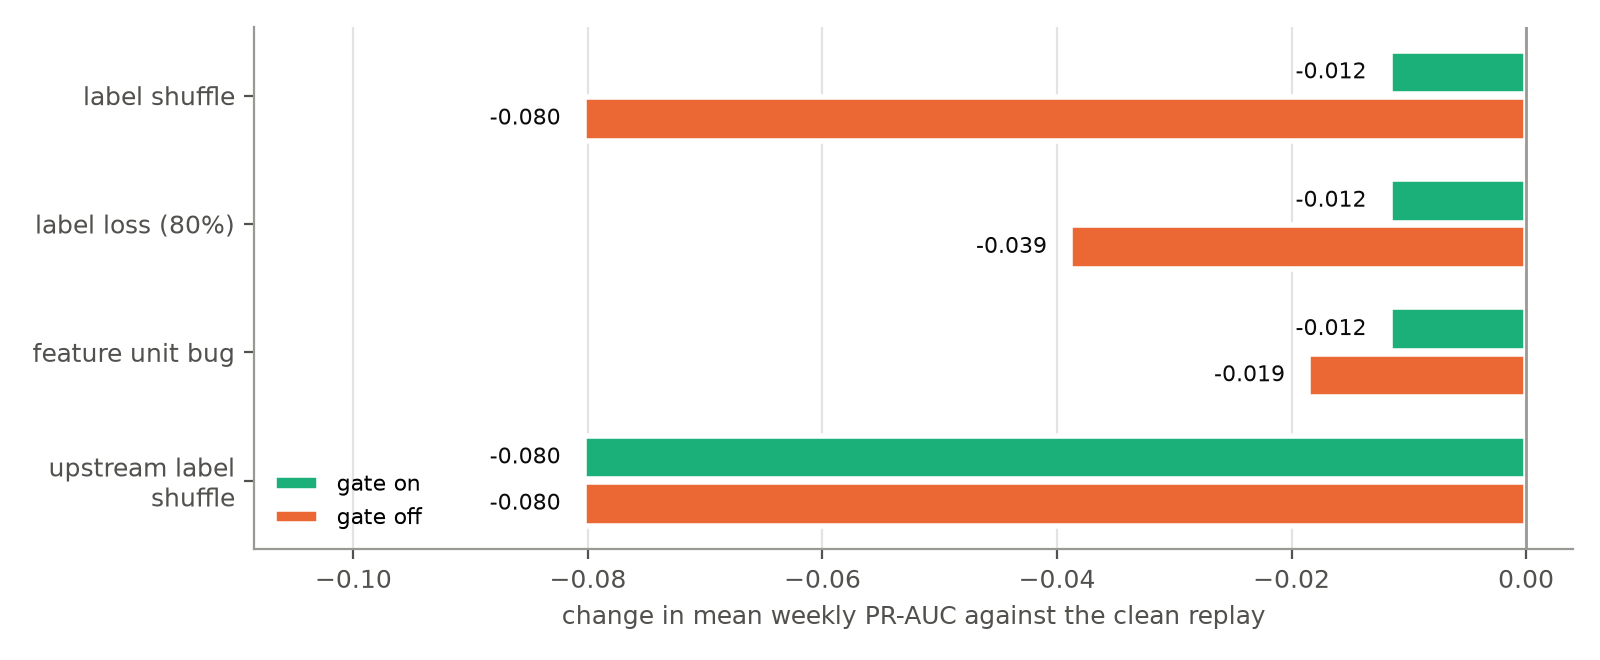
\includegraphics[width=\textwidth]{figures/results_gate.png}
  \caption{Fault injection on IEEE-CIS: change in mean weekly PR-AUC against a clean replay when two retraining jobs are faulty, with the promotion gate on and off}
  \label{fig:gate}
\end{figure}

The upstream fault, which corrupts the label store that the gate itself reads, passed the gate as expected, since both models looked equally poor on corrupted labels. Here the safety net took over: seven days after each faulty promotion, the live PR-AUC on matured labels had fallen to 0.045 and 0.036, below both 70\% of the reference and three times the fraud rate, and the framework retrained early. The damage was limited to one week per fault (-0.080 in total). Before the reference of the safety net included recent live performance (Section \ref{sec:safety}), the same fault went undetected and cost -0.149.

\textbf{Answer to RQ4.} Yes. Built on the findings of RQ1 to RQ3, the framework sustained the performance of the best offline policy in a full replay, prevented every faulty model it could observe from reaching production, recovered within a week from the fault it could not observe, and, with automatic window selection, performed at or near the best fixed window on all three datasets.

\section{Final Design Adjustments}\label{sec:adjust}

Three changes were made to the design during the evaluation, each prompted by a result.

\subsection{Promotion Gate on Production Features}\label{sec:adj_gate}

The first version of the promotion gate compared the challenger and the champion using scores stored when each model was trained. A fault test with a feature unit bug showed the weakness of this: a model trained on wrongly scaled features looks good on equally wrong validation data. The gate was changed to re-score both models through the production feature path (Section \ref{sec:gate}), after which it rejected the faulty models.

\subsection{Safety-Net Reference from Live Performance}\label{sec:adj_safety}

Originally the safety net compared live PR-AUC with the model's own validation PR-AUC. When the label store itself was corrupted, a faulty model reported a poor validation score and was then judged against that low bar, so the fault went undetected and cost 0.149 PR-AUC. The reference was changed to the better of the validation score and the median of the last four live measurements, and a no-skill check was added (Section \ref{sec:safety}); the same fault was then caught after seven days and cost 0.080.

\subsection{Automatic Training-Window Selection}\label{sec:adj_window}

\textbf{Automatic window selection.} No fixed window suited all three datasets: the 60-day window was best on IEEE-CIS (0.529) but lost 0.172 against the static model on Sparkov, while all history was best on Sparkov and BAF but only second on IEEE-CIS. With automatic selection, the framework chose the 60-day window at all five retrains on IEEE-CIS and all history at all 25 retrains on Sparkov, matching the best fixed window on both (difference 0.000 and -0.0002). On BAF it chose the 60-day window at the first two retrains, when the two candidates were close and the shorter window scored slightly higher on recent data, and all history at the remaining seven. It ended 0.0045 below the best fixed window on BAF, a small but reliable difference (95\% interval over weeks -0.008 to -0.001), and 0.004 above the static model. Figure \ref{fig:window} shows that the automatic setting avoided the large loss of a wrongly chosen window on every dataset without knowing in advance which window suited the data.

\begin{figure}[htbp]
  \centering
  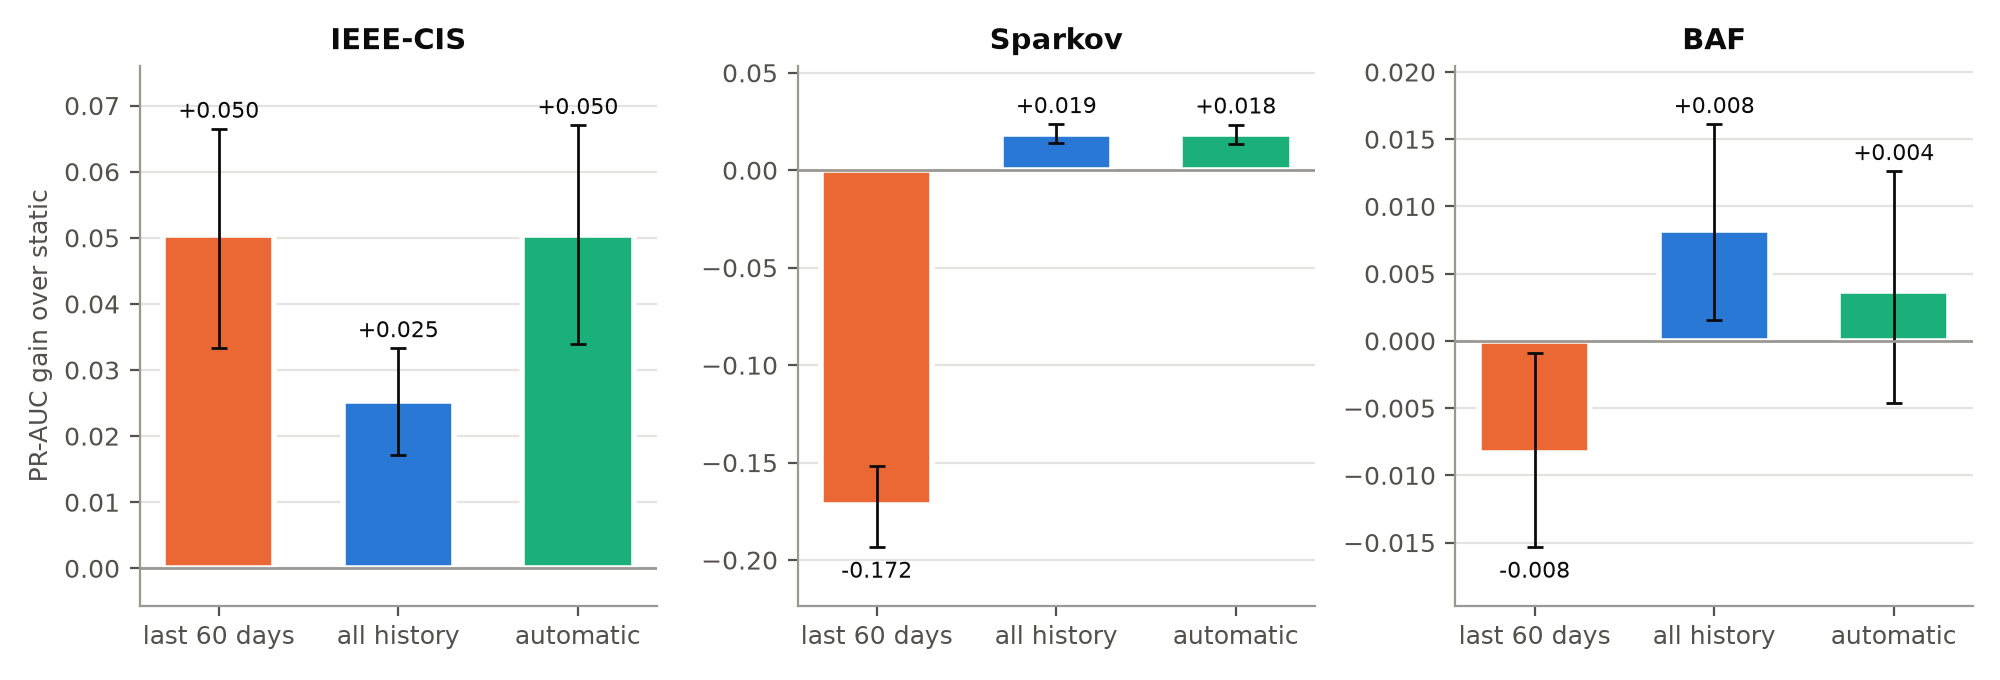
\includegraphics[width=\textwidth]{figures/results_window.png}
  \caption{Framework replays (30-day label delay): gain in mean weekly PR-AUC over the static model for each training-window choice, with 95\% bootstrap intervals over weeks}
  \label{fig:window}
\end{figure}

\section{Summary of Results}\label{sec:summary}

Table \ref{tab:answers} summarises the answers to the research questions. Taken together, the results support the design of the proposed framework: performance is monitored on delayed labels rather than inferred from drift, retraining follows a schedule rather than a drift alarm, the training window is selected from the data, and every new model must pass a promotion gate. Section \ref{sec:discussion} discusses what these results mean, how they relate to earlier work, and where they are limited.

{\footnotesize
\begin{longtable}{>{\raggedright\arraybackslash}p{0.09\textwidth}>{\raggedright\arraybackslash}p{0.85\textwidth}}
\caption{Answers to the research questions}\label{tab:answers}\\
\toprule
\textbf{RQ} & \textbf{Answer} \\
\midrule
\endfirsthead
\toprule
\textbf{RQ} & \textbf{Answer} \\
\midrule
\endhead
RQ1 & Performance after deployment changed differently on each dataset: it fell by a third on IEEE-CIS but stayed stable on Sparkov and BAF. Label-free drift measures did not reflect this: input and score drift stayed low while IEEE-CIS decayed, and input drift was strong (PSI up to 4.6) while Sparkov and BAF did not. \\ \midrule
RQ2 & Scheduled retraining improved performance on every dataset when its window suited the data, with gains of 0.008 to 0.078 PR-AUC. On IEEE-CIS the gain shrank from 0.078 to 0.010 as the label delay grew from 0 to 60 days. \\ \midrule
RQ3 & No. Tuned fairly with walk-forward tuning, drift-triggered retraining was worse than scheduled retraining in 7 of 9 comparisons and never better beyond noise; it retrained less often. The training window mattered more than the trigger. \\ \midrule
RQ4 & Yes. The framework reproduced the offline results within 0.002 PR-AUC, blocked every faulty model the gate could observe, limited the damage of the unobservable fault through the safety net, and, with automatic window selection, matched the best fixed window on two datasets and came within 0.005 on the third. \\ \bottomrule
\end{longtable}
}

\section{Statistical Analysis}\label{sec:statistics}

Three layers of statistical analysis support the results. First, every comparison between strategies is paired: all strategies are evaluated on the same weeks and the same bootstrap resamples, which removes most of the noise they share. Second, the paired day-block bootstrap resamples whole days within each week, which respects the correlation between transactions of the same day, and yields the 95\% intervals reported throughout. Third, training randomness is covered by repeating the key comparisons with five LightGBM seeds.

{\footnotesize
\begin{longtable}{>{\raggedright\arraybackslash}p{0.12\textwidth}>{\raggedright\arraybackslash}p{0.08\textwidth}>{\raggedright\arraybackslash}p{0.24\textwidth}>{\raggedright\arraybackslash}p{0.24\textwidth}>{\raggedright\arraybackslash}p{0.24\textwidth}}
\caption{Key differences over five training seeds (mean, and the number of seeds in which the difference is positive). Best schedule: last 60 days on IEEE-CIS, all history on Sparkov and BAF}\label{tab:seeds}\\
\toprule
\textbf{Dataset} & \textbf{Delay} & \textbf{All history - static} & \textbf{Last 60 days - static} & \textbf{Default drift trigger - best schedule} \\
\midrule
\endfirsthead
\toprule
\textbf{Dataset} & \textbf{Delay} & \textbf{All history - static} & \textbf{Last 60 days - static} & \textbf{Default drift trigger - best schedule} \\
\midrule
\endhead
IEEE-CIS & 0 d & +0.033 (5/5) & +0.080 (5/5) & -0.055 (0/5) \\ \midrule
 & 30 d & +0.022 (5/5) & +0.046 (5/5) & -0.026 (0/5) \\ \midrule
Sparkov & 0 d & +0.012 (5/5) & -0.194 (0/5) & -0.012 (0/5) \\ \midrule
 & 30 d & +0.016 (5/5) & -0.171 (0/5) & -0.016 (0/5) \\ \midrule
BAF & 0 d & +0.006 (5/5) & -0.006 (0/5) & -0.006 (0/5) \\ \midrule
 & 30 d & +0.009 (5/5) & -0.007 (0/5) & -0.009 (0/5) \\ \bottomrule
\end{longtable}
}

\textbf{The results are not due to training randomness.} Table \ref{tab:seeds} repeats the key comparisons with five LightGBM seeds. Every difference in the table had the same sign in all five seeds on every dataset. The spread of a single configuration across seeds was small compared with the differences between strategies: the median standard deviation was 0.004 on IEEE-CIS, 0.010 on Sparkov and 0.003 on BAF.

Because many comparisons are reported, a single interval that excludes zero should not be over-interpreted. The conclusions of this thesis rest instead on patterns that hold across label delays, datasets, seeds and analyses: for example, the drift trigger was reliably worse than the schedule in seven of nine walk-forward comparisons and never reliably better in any of them, and the equal-budget analysis pointed the same way whenever labels were delayed.

\section{Discussions}\label{sec:discussion}

\textbf{Drift indicators and delayed labels.} The central finding is that label-free drift indicators did not reflect what mattered. They stayed quiet while the IEEE-CIS model lost a third of its PR-AUC, and they signalled strong drift on Sparkov and BAF while the models were unaffected. Shakil et al. noted that statistical drift does not always mean lower performance \cite{shakil2025}; on natural drift in fraud data we observed this in both directions. For a fraud system this means that drift alarms should inform investigation, not trigger retraining, and that the performance on matured labels is the signal to watch, even though it arrives late. This is the sense in which the framework is drift-aware.

\textbf{Schedules and triggers.} Earlier work reported that drift-triggered retraining matches or beats a schedule with fewer retrains \cite{wong2025,yelleti2025}. Those results were obtained with injected drift or immediate labels. Under realistic label delay a performance trigger can only react after a drop has been confirmed on labels that are weeks old, and a label-free trigger reacts to the wrong signal. A schedule needs no evidence and keeps the model fresh, and the equal-budget analysis shows that under label delay its advantage is not merely a matter of retraining more often. With immediate labels, a trigger could be the more economical policy, as on BAF, which explains why earlier studies that assumed immediate labels favoured triggers. The result is consistent with Dal Pozzolo et al., who stressed that verification latency shapes how a fraud model can be updated \cite{dalpozzolo2018}, and with Amekoe et al., who found that batch models retrained on delayed labels remain competitive \cite{amekoe2024}.

\textbf{The training window.} The choice of training window changed results by up to 0.26 PR-AUC, far more than the choice of trigger. Recent data was best on IEEE-CIS, which decays, and all history was best on Sparkov and BAF, which are stable and have few frauds. Because no fixed window suits every deployment, selecting the window from the data, as the framework now does, is a practical way to avoid a costly wrong choice.

\textbf{Safe automation.} Automated retraining will eventually train on bad data. The fault tests show that a promotion gate that re-scores models on production data stops faults it can observe, and that a safety net based on live performance limits the damage of faults it cannot. Closed-loop MLOps frameworks such as HAMF \cite{reda2025} automate the loop; this thesis adds evidence on how such safeguards behave when labels arrive late.

\textbf{Limitations.} The deployment is replayed from historical data, so live latency and the behaviour of a real chargeback feed are not observed, and every label arrives after the same delay, without faster investigator feedback. One model family is used throughout. IEEE-CIS covers only six months, Sparkov is simulated, and BAF records only the month of each application, so drift within a month cannot appear. The equal-budget comparison is complete on IEEE-CIS and BAF and under way on Sparkov, and the scoring service has not yet been load tested.
